% Important: If latex complains about unicode characters,
% please use "\usepackage[utf8x]{inputenc}" in your preamble
% You can change the size of the picture by putting it into the construct:
% 1) \resizebox{10cm}{!}{"below picture"} to scale horizontally to 10 cm
% 2) \resizebox{!}{15cm}{"below picture"} to scale vertically to 15 cm
% 3) \resizebox{10cm}{15cm}{"below picture"} a combination of above two
% It is not recomended to use the scale option of the tikzpicture environment.
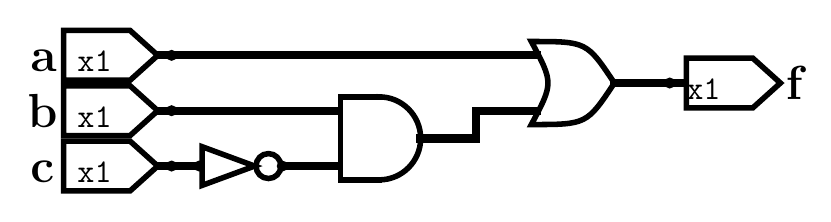
\begin{tikzpicture}[x=1pt,y=-1pt,line cap=rect]
\def\logisimfontA#1{\fontfamily{cmr}{#1}} % Replaced by logisim, original font was "SansSerif"
\def\logisimfontB#1{\fontfamily{cmtt}{#1}} % Replaced by logisim, original font was "Monospaced"
\definecolor{custcol_0_0_0}{RGB}{0, 0, 0}
\definecolor{custcol_ff_ff_ff}{RGB}{255, 255, 255}
\draw [line width=3.0pt, custcol_0_0_0 ]  (217.0,25.0) -- (237.0,25.0) ;
\draw [line width=3.0pt, custcol_0_0_0 ]  (97.0,55.0) -- (117.0,55.0) ;
\draw [line width=3.0pt, custcol_0_0_0 ]  (52.0,55.0) -- (57.0,55.0) -- (67.0,55.0) ;
\draw [line width=2.0pt, custcol_0_0_0 ]  (42.0,64.0) -- (52.0,55.0) -- (42.0,46.0) -- (18.0,46.0) -- (18.0,64.0) -- cycle;
\logisimfontB{\fontsize{12pt}{12pt}\selectfont\node[inner sep=0, outer sep=0, custcol_0_0_0, anchor=base west] at  (23.0,61.0)  {x1};}
\logisimfontA{\fontsize{16pt}{16pt}\fontseries{bx}\selectfont\node[inner sep=0, outer sep=0, custcol_0_0_0, anchor=base west] at  (6.0,61.0)  {c};}
\fill [line width=2.0pt, custcol_0_0_0]  (57.0,55.0) ellipse (2.0 and 2.0 );
\draw [line width=3.0pt, custcol_0_0_0 ]  (52.0,35.0) -- (57.0,35.0) -- (117.0,35.0) ;
\draw [line width=2.0pt, custcol_0_0_0 ]  (42.0,44.0) -- (52.0,35.0) -- (42.0,26.0) -- (18.0,26.0) -- (18.0,44.0) -- cycle;
\logisimfontB{\fontsize{12pt}{12pt}\selectfont\node[inner sep=0, outer sep=0, custcol_0_0_0, anchor=base west] at  (23.0,41.0)  {x1};}
\logisimfontA{\fontsize{16pt}{16pt}\fontseries{bx}\selectfont\node[inner sep=0, outer sep=0, custcol_0_0_0, anchor=base west] at  (5.0,41.0)  {b};}
\fill [line width=2.0pt, custcol_0_0_0]  (57.0,35.0) ellipse (2.0 and 2.0 );
\draw [line width=2.0pt, custcol_0_0_0 ]  (42.0,24.0) -- (52.0,15.0) -- (42.0,6.0) -- (18.0,6.0) -- (18.0,24.0) -- cycle;
\logisimfontB{\fontsize{12pt}{12pt}\selectfont\node[inner sep=0, outer sep=0, custcol_0_0_0, anchor=base west] at  (23.0,21.0)  {x1};}
\logisimfontA{\fontsize{16pt}{16pt}\fontseries{bx}\selectfont\node[inner sep=0, outer sep=0, custcol_0_0_0, anchor=base west] at  (6.0,21.0)  {a};}
\fill [line width=2.0pt, custcol_0_0_0]  (57.0,15.0) ellipse (2.0 and 2.0 );
\draw [line width=2.0pt, custcol_0_0_0 ]  (87.0,55.0) -- (68.0,48.0) -- (68.0,62.0) -- cycle;
\draw [line width=2.0pt, custcol_0_0_0]  (92.0,55.0) ellipse (4.5 and 4.5 );
\fill [line width=2.0pt, custcol_0_0_0]  (97.0,55.0) ellipse (2.0 and 2.0 );
\fill [line width=2.0pt, custcol_0_0_0]  (67.0,55.0) ellipse (2.0 and 2.0 );
\draw [line width=3.0pt, custcol_0_0_0 ]  (52.0,15.0) -- (57.0,15.0) -- (187.0,15.0) -- (189.0,15.0) ;
\draw [line width=3.0pt, custcol_0_0_0 ]  (147.0,45.0) -- (167.0,45.0) -- (167.0,35.0) -- (187.0,35.0) -- (189.0,35.0) ;
\draw [line width=2.0pt, custcol_0_0_0 ]  (217.0,25.0) .. controls  (207.0,10.0)  ..  (187.0,10.0) .. controls  (195.0,25.0)  ..  (187.0,40.0) .. controls  (207.0,40.0)  ..  (217.0,25.0) -- cycle ;
\draw [line width=3.0pt, custcol_0_0_0 ]  (241.0,25.0) -- (238.0,25.0) ;
\draw [line width=2.0pt, custcol_0_0_0 ]  (267.0,16.0) -- (277.0,25.0) -- (267.0,34.0) -- (243.0,34.0) -- (243.0,16.0) -- cycle;
\logisimfontB{\fontsize{12pt}{12pt}\selectfont\node[inner sep=0, outer sep=0, custcol_0_0_0, anchor=base west] at  (243.0,31.0)  {x1};}
\logisimfontA{\fontsize{16pt}{16pt}\fontseries{bx}\selectfont\node[inner sep=0, outer sep=0, custcol_0_0_0, anchor=base west] at  (279.0,31.0)  {f};}
\fill [line width=2.0pt, custcol_0_0_0]  (237.0,25.0) ellipse (2.0 and 2.0 );
\draw [line width=2.0pt, custcol_0_0_0] (132.0,60.0) arc (90.0:-90.0:15.0 and 15.0 );
\draw [line width=2.0pt, custcol_0_0_0 ]  (132.0,30.0) -- (118.0,30.0) -- (118.0,60.0) -- (132.0,60.0) ;
\end{tikzpicture}

